% Created by tikzDevice version 0.12.6 on 2025-07-29 11:39:25
% !TEX encoding = UTF-8 Unicode
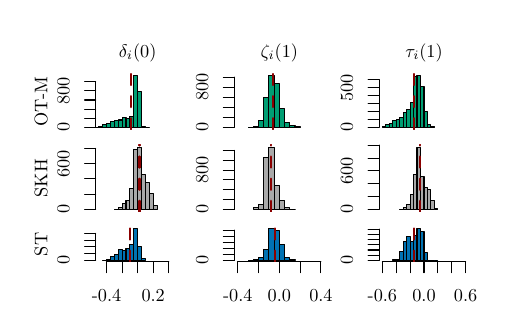
\begin{tikzpicture}[x=1pt,y=1pt]
\definecolor{fillColor}{RGB}{255,255,255}
\path[use as bounding box,fill=fillColor,fill opacity=0.00] (0,0) rectangle (162.61,101.18);
\begin{scope}
\path[clip] ( 24.55, 64.46) rectangle ( 54.91, 84.55);
\definecolor{drawColor}{RGB}{0,0,0}
\definecolor{fillColor}{RGB}{0,158,115}

\path[draw=drawColor,line width= 0.4pt,line join=round,line cap=round,fill=fillColor] ( 24.27, 65.21) rectangle ( 25.68, 65.22);

\path[draw=drawColor,line width= 0.4pt,line join=round,line cap=round,fill=fillColor] ( 25.68, 65.21) rectangle ( 27.08, 65.34);

\path[draw=drawColor,line width= 0.4pt,line join=round,line cap=round,fill=fillColor] ( 27.08, 65.21) rectangle ( 28.49, 66.31);

\path[draw=drawColor,line width= 0.4pt,line join=round,line cap=round,fill=fillColor] ( 28.49, 65.21) rectangle ( 29.89, 66.55);

\path[draw=drawColor,line width= 0.4pt,line join=round,line cap=round,fill=fillColor] ( 29.89, 65.21) rectangle ( 31.30, 67.31);

\path[draw=drawColor,line width= 0.4pt,line join=round,line cap=round,fill=fillColor] ( 31.30, 65.21) rectangle ( 32.70, 67.68);

\path[draw=drawColor,line width= 0.4pt,line join=round,line cap=round,fill=fillColor] ( 32.70, 65.21) rectangle ( 34.11, 67.83);

\path[draw=drawColor,line width= 0.4pt,line join=round,line cap=round,fill=fillColor] ( 34.11, 65.21) rectangle ( 35.51, 68.62);

\path[draw=drawColor,line width= 0.4pt,line join=round,line cap=round,fill=fillColor] ( 35.51, 65.21) rectangle ( 36.92, 68.49);

\path[draw=drawColor,line width= 0.4pt,line join=round,line cap=round,fill=fillColor] ( 36.92, 65.21) rectangle ( 38.32, 69.24);

\path[draw=drawColor,line width= 0.4pt,line join=round,line cap=round,fill=fillColor] ( 38.32, 65.21) rectangle ( 39.73, 83.80);

\path[draw=drawColor,line width= 0.4pt,line join=round,line cap=round,fill=fillColor] ( 39.73, 65.21) rectangle ( 41.13, 77.96);

\path[draw=drawColor,line width= 0.4pt,line join=round,line cap=round,fill=fillColor] ( 41.13, 65.21) rectangle ( 42.54, 65.37);

\path[draw=drawColor,line width= 0.4pt,line join=round,line cap=round,fill=fillColor] ( 42.54, 65.21) rectangle ( 43.94, 65.24);
\end{scope}
\begin{scope}
\path[clip] (  0.00,  0.00) rectangle (162.61,101.18);
\definecolor{drawColor}{RGB}{0,0,0}

\path[draw=drawColor,line width= 0.4pt,line join=round,line cap=round] ( 24.55, 65.21) -- ( 24.55, 81.60);

\path[draw=drawColor,line width= 0.4pt,line join=round,line cap=round] ( 24.55, 65.21) -- ( 20.59, 65.21);

\path[draw=drawColor,line width= 0.4pt,line join=round,line cap=round] ( 24.55, 68.49) -- ( 20.59, 68.49);

\path[draw=drawColor,line width= 0.4pt,line join=round,line cap=round] ( 24.55, 71.77) -- ( 20.59, 71.77);

\path[draw=drawColor,line width= 0.4pt,line join=round,line cap=round] ( 24.55, 75.05) -- ( 20.59, 75.05);

\path[draw=drawColor,line width= 0.4pt,line join=round,line cap=round] ( 24.55, 78.33) -- ( 20.59, 78.33);

\path[draw=drawColor,line width= 0.4pt,line join=round,line cap=round] ( 24.55, 81.60) -- ( 20.59, 81.60);

\node[text=drawColor,rotate= 90.00,anchor=base,inner sep=0pt, outer sep=0pt, scale=  0.66] at ( 15.05, 65.21) {0};

\node[text=drawColor,rotate= 90.00,anchor=base,inner sep=0pt, outer sep=0pt, scale=  0.66] at ( 15.05, 78.33) {800};
\end{scope}
\begin{scope}
\path[clip] (  0.00, 59.71) rectangle ( 58.07,101.18);
\definecolor{drawColor}{RGB}{0,0,0}

\node[text=drawColor,anchor=base,inner sep=0pt, outer sep=0pt, scale=  0.66] at ( 39.73, 90.58) {\bfseries $\delta_i(0)$};

\node[text=drawColor,rotate= 90.00,anchor=base,inner sep=0pt, outer sep=0pt, scale=  0.66] at (  7.13, 74.50) {OT-M};
\end{scope}
\begin{scope}
\path[clip] ( 24.55, 64.46) rectangle ( 54.91, 84.55);
\definecolor{drawColor}{RGB}{139,0,0}

\path[draw=drawColor,line width= 0.8pt,dash pattern=on 4pt off 4pt ,line join=round,line cap=round] ( 37.34, 64.46) -- ( 37.34, 84.55);
\end{scope}
\begin{scope}
\path[clip] ( 74.71, 64.46) rectangle (107.17, 84.55);
\definecolor{drawColor}{RGB}{0,0,0}
\definecolor{fillColor}{RGB}{0,158,115}

\path[draw=drawColor,line width= 0.4pt,line join=round,line cap=round,fill=fillColor] ( 79.67, 65.21) rectangle ( 81.55, 65.23);

\path[draw=drawColor,line width= 0.4pt,line join=round,line cap=round,fill=fillColor] ( 81.55, 65.21) rectangle ( 83.42, 65.57);

\path[draw=drawColor,line width= 0.4pt,line join=round,line cap=round,fill=fillColor] ( 83.42, 65.21) rectangle ( 85.30, 67.72);

\path[draw=drawColor,line width= 0.4pt,line join=round,line cap=round,fill=fillColor] ( 85.30, 65.21) rectangle ( 87.18, 76.09);

\path[draw=drawColor,line width= 0.4pt,line join=round,line cap=round,fill=fillColor] ( 87.18, 65.21) rectangle ( 89.06, 83.80);

\path[draw=drawColor,line width= 0.4pt,line join=round,line cap=round,fill=fillColor] ( 89.06, 65.21) rectangle ( 90.94, 81.16);

\path[draw=drawColor,line width= 0.4pt,line join=round,line cap=round,fill=fillColor] ( 90.94, 65.21) rectangle ( 92.82, 71.89);

\path[draw=drawColor,line width= 0.4pt,line join=round,line cap=round,fill=fillColor] ( 92.82, 65.21) rectangle ( 94.70, 66.96);

\path[draw=drawColor,line width= 0.4pt,line join=round,line cap=round,fill=fillColor] ( 94.70, 65.21) rectangle ( 96.58, 65.75);

\path[draw=drawColor,line width= 0.4pt,line join=round,line cap=round,fill=fillColor] ( 96.58, 65.21) rectangle ( 98.45, 65.28);
\end{scope}
\begin{scope}
\path[clip] (  0.00,  0.00) rectangle (162.61,101.18);
\definecolor{drawColor}{RGB}{0,0,0}

\path[draw=drawColor,line width= 0.4pt,line join=round,line cap=round] ( 74.71, 65.21) -- ( 74.71, 83.28);

\path[draw=drawColor,line width= 0.4pt,line join=round,line cap=round] ( 74.71, 65.21) -- ( 70.75, 65.21);

\path[draw=drawColor,line width= 0.4pt,line join=round,line cap=round] ( 74.71, 68.82) -- ( 70.75, 68.82);

\path[draw=drawColor,line width= 0.4pt,line join=round,line cap=round] ( 74.71, 72.44) -- ( 70.75, 72.44);

\path[draw=drawColor,line width= 0.4pt,line join=round,line cap=round] ( 74.71, 76.05) -- ( 70.75, 76.05);

\path[draw=drawColor,line width= 0.4pt,line join=round,line cap=round] ( 74.71, 79.66) -- ( 70.75, 79.66);

\path[draw=drawColor,line width= 0.4pt,line join=round,line cap=round] ( 74.71, 83.28) -- ( 70.75, 83.28);

\node[text=drawColor,rotate= 90.00,anchor=base,inner sep=0pt, outer sep=0pt, scale=  0.66] at ( 65.20, 65.21) {0};

\node[text=drawColor,rotate= 90.00,anchor=base,inner sep=0pt, outer sep=0pt, scale=  0.66] at ( 65.20, 79.66) {800};
\end{scope}
\begin{scope}
\path[clip] ( 58.07, 59.71) rectangle (110.34,101.18);
\definecolor{drawColor}{RGB}{0,0,0}

\node[text=drawColor,anchor=base,inner sep=0pt, outer sep=0pt, scale=  0.66] at ( 90.94, 90.58) {\bfseries $\zeta_i(1)$};
\end{scope}
\begin{scope}
\path[clip] ( 74.71, 64.46) rectangle (107.17, 84.55);
\definecolor{drawColor}{RGB}{139,0,0}

\path[draw=drawColor,line width= 0.8pt,dash pattern=on 4pt off 4pt ,line join=round,line cap=round] ( 88.75, 64.46) -- ( 88.75, 84.55);
\end{scope}
\begin{scope}
\path[clip] (126.97, 64.46) rectangle (159.44, 84.55);
\definecolor{drawColor}{RGB}{0,0,0}
\definecolor{fillColor}{RGB}{0,158,115}

\path[draw=drawColor,line width= 0.4pt,line join=round,line cap=round,fill=fillColor] (128.18, 65.21) rectangle (129.43, 65.49);

\path[draw=drawColor,line width= 0.4pt,line join=round,line cap=round,fill=fillColor] (129.43, 65.21) rectangle (130.68, 66.21);

\path[draw=drawColor,line width= 0.4pt,line join=round,line cap=round,fill=fillColor] (130.68, 65.21) rectangle (131.93, 66.69);

\path[draw=drawColor,line width= 0.4pt,line join=round,line cap=round,fill=fillColor] (131.93, 65.21) rectangle (133.19, 67.58);

\path[draw=drawColor,line width= 0.4pt,line join=round,line cap=round,fill=fillColor] (133.19, 65.21) rectangle (134.44, 68.10);

\path[draw=drawColor,line width= 0.4pt,line join=round,line cap=round,fill=fillColor] (134.44, 65.21) rectangle (135.69, 68.84);

\path[draw=drawColor,line width= 0.4pt,line join=round,line cap=round,fill=fillColor] (135.69, 65.21) rectangle (136.94, 70.47);

\path[draw=drawColor,line width= 0.4pt,line join=round,line cap=round,fill=fillColor] (136.94, 65.21) rectangle (138.20, 71.67);

\path[draw=drawColor,line width= 0.4pt,line join=round,line cap=round,fill=fillColor] (138.20, 65.21) rectangle (139.45, 74.30);

\path[draw=drawColor,line width= 0.4pt,line join=round,line cap=round,fill=fillColor] (139.45, 65.21) rectangle (140.70, 83.60);

\path[draw=drawColor,line width= 0.4pt,line join=round,line cap=round,fill=fillColor] (140.70, 65.21) rectangle (141.95, 83.80);

\path[draw=drawColor,line width= 0.4pt,line join=round,line cap=round,fill=fillColor] (141.95, 65.21) rectangle (143.21, 79.97);

\path[draw=drawColor,line width= 0.4pt,line join=round,line cap=round,fill=fillColor] (143.21, 65.21) rectangle (144.46, 70.73);

\path[draw=drawColor,line width= 0.4pt,line join=round,line cap=round,fill=fillColor] (144.46, 65.21) rectangle (145.71, 66.07);

\path[draw=drawColor,line width= 0.4pt,line join=round,line cap=round,fill=fillColor] (145.71, 65.21) rectangle (146.96, 65.41);
\end{scope}
\begin{scope}
\path[clip] (  0.00,  0.00) rectangle (162.61,101.18);
\definecolor{drawColor}{RGB}{0,0,0}

\path[draw=drawColor,line width= 0.4pt,line join=round,line cap=round] (126.97, 65.21) -- (126.97, 82.37);

\path[draw=drawColor,line width= 0.4pt,line join=round,line cap=round] (126.97, 65.21) -- (123.01, 65.21);

\path[draw=drawColor,line width= 0.4pt,line join=round,line cap=round] (126.97, 68.07) -- (123.01, 68.07);

\path[draw=drawColor,line width= 0.4pt,line join=round,line cap=round] (126.97, 70.93) -- (123.01, 70.93);

\path[draw=drawColor,line width= 0.4pt,line join=round,line cap=round] (126.97, 73.79) -- (123.01, 73.79);

\path[draw=drawColor,line width= 0.4pt,line join=round,line cap=round] (126.97, 76.65) -- (123.01, 76.65);

\path[draw=drawColor,line width= 0.4pt,line join=round,line cap=round] (126.97, 79.51) -- (123.01, 79.51);

\path[draw=drawColor,line width= 0.4pt,line join=round,line cap=round] (126.97, 82.37) -- (123.01, 82.37);

\node[text=drawColor,rotate= 90.00,anchor=base,inner sep=0pt, outer sep=0pt, scale=  0.66] at (117.47, 65.21) {0};

\node[text=drawColor,rotate= 90.00,anchor=base,inner sep=0pt, outer sep=0pt, scale=  0.66] at (117.47, 79.51) {500};
\end{scope}
\begin{scope}
\path[clip] (110.34, 59.71) rectangle (162.61,101.18);
\definecolor{drawColor}{RGB}{0,0,0}

\node[text=drawColor,anchor=base,inner sep=0pt, outer sep=0pt, scale=  0.66] at (143.21, 90.58) {\bfseries $\tau_i(1)$};
\end{scope}
\begin{scope}
\path[clip] (126.97, 64.46) rectangle (159.44, 84.55);
\definecolor{drawColor}{RGB}{139,0,0}

\path[draw=drawColor,line width= 0.8pt,dash pattern=on 4pt off 4pt ,line join=round,line cap=round] (139.62, 64.46) -- (139.62, 84.55);
\end{scope}
\begin{scope}
\path[clip] ( 24.55, 34.61) rectangle ( 54.91, 58.92);
\definecolor{drawColor}{RGB}{0,0,0}
\definecolor{fillColor}{RGB}{169,169,169}

\path[draw=drawColor,line width= 0.4pt,line join=round,line cap=round,fill=fillColor] ( 31.30, 35.51) rectangle ( 32.70, 35.54);

\path[draw=drawColor,line width= 0.4pt,line join=round,line cap=round,fill=fillColor] ( 32.70, 35.51) rectangle ( 34.11, 36.28);

\path[draw=drawColor,line width= 0.4pt,line join=round,line cap=round,fill=fillColor] ( 34.11, 35.51) rectangle ( 35.51, 37.74);

\path[draw=drawColor,line width= 0.4pt,line join=round,line cap=round,fill=fillColor] ( 35.51, 35.51) rectangle ( 36.92, 38.87);

\path[draw=drawColor,line width= 0.4pt,line join=round,line cap=round,fill=fillColor] ( 36.92, 35.51) rectangle ( 38.32, 42.92);

\path[draw=drawColor,line width= 0.4pt,line join=round,line cap=round,fill=fillColor] ( 38.32, 35.51) rectangle ( 39.73, 57.14);

\path[draw=drawColor,line width= 0.4pt,line join=round,line cap=round,fill=fillColor] ( 39.73, 35.51) rectangle ( 41.13, 58.02);

\path[draw=drawColor,line width= 0.4pt,line join=round,line cap=round,fill=fillColor] ( 41.13, 35.51) rectangle ( 42.54, 48.16);

\path[draw=drawColor,line width= 0.4pt,line join=round,line cap=round,fill=fillColor] ( 42.54, 35.51) rectangle ( 43.94, 45.23);

\path[draw=drawColor,line width= 0.4pt,line join=round,line cap=round,fill=fillColor] ( 43.94, 35.51) rectangle ( 45.35, 41.13);

\path[draw=drawColor,line width= 0.4pt,line join=round,line cap=round,fill=fillColor] ( 45.35, 35.51) rectangle ( 46.76, 37.05);
\end{scope}
\begin{scope}
\path[clip] (  0.00,  0.00) rectangle (162.61,101.18);
\definecolor{drawColor}{RGB}{0,0,0}

\path[draw=drawColor,line width= 0.4pt,line join=round,line cap=round] ( 24.55, 35.51) -- ( 24.55, 57.55);

\path[draw=drawColor,line width= 0.4pt,line join=round,line cap=round] ( 24.55, 35.51) -- ( 20.59, 35.51);

\path[draw=drawColor,line width= 0.4pt,line join=round,line cap=round] ( 24.55, 41.02) -- ( 20.59, 41.02);

\path[draw=drawColor,line width= 0.4pt,line join=round,line cap=round] ( 24.55, 46.53) -- ( 20.59, 46.53);

\path[draw=drawColor,line width= 0.4pt,line join=round,line cap=round] ( 24.55, 52.04) -- ( 20.59, 52.04);

\path[draw=drawColor,line width= 0.4pt,line join=round,line cap=round] ( 24.55, 57.55) -- ( 20.59, 57.55);

\node[text=drawColor,rotate= 90.00,anchor=base,inner sep=0pt, outer sep=0pt, scale=  0.66] at ( 15.05, 35.51) {0};

\node[text=drawColor,rotate= 90.00,anchor=base,inner sep=0pt, outer sep=0pt, scale=  0.66] at ( 15.05, 52.04) {600};
\end{scope}
\begin{scope}
\path[clip] (  0.00, 29.86) rectangle ( 58.07, 59.71);
\definecolor{drawColor}{RGB}{0,0,0}

\node[text=drawColor,rotate= 90.00,anchor=base,inner sep=0pt, outer sep=0pt, scale=  0.66] at (  7.13, 46.76) {SKH};
\end{scope}
\begin{scope}
\path[clip] ( 24.55, 34.61) rectangle ( 54.91, 58.92);
\definecolor{drawColor}{RGB}{139,0,0}

\path[draw=drawColor,line width= 0.8pt,dash pattern=on 4pt off 4pt ,line join=round,line cap=round] ( 40.37, 34.61) -- ( 40.37, 58.92);
\end{scope}
\begin{scope}
\path[clip] ( 74.71, 34.61) rectangle (107.17, 58.92);
\definecolor{drawColor}{RGB}{0,0,0}
\definecolor{fillColor}{RGB}{169,169,169}

\path[draw=drawColor,line width= 0.4pt,line join=round,line cap=round,fill=fillColor] ( 81.55, 35.51) rectangle ( 83.42, 36.04);

\path[draw=drawColor,line width= 0.4pt,line join=round,line cap=round,fill=fillColor] ( 83.42, 35.51) rectangle ( 85.30, 37.39);

\path[draw=drawColor,line width= 0.4pt,line join=round,line cap=round,fill=fillColor] ( 85.30, 35.51) rectangle ( 87.18, 54.38);

\path[draw=drawColor,line width= 0.4pt,line join=round,line cap=round,fill=fillColor] ( 87.18, 35.51) rectangle ( 89.06, 58.02);

\path[draw=drawColor,line width= 0.4pt,line join=round,line cap=round,fill=fillColor] ( 89.06, 35.51) rectangle ( 90.94, 44.18);

\path[draw=drawColor,line width= 0.4pt,line join=round,line cap=round,fill=fillColor] ( 90.94, 35.51) rectangle ( 92.82, 38.78);

\path[draw=drawColor,line width= 0.4pt,line join=round,line cap=round,fill=fillColor] ( 92.82, 35.51) rectangle ( 94.70, 36.09);

\path[draw=drawColor,line width= 0.4pt,line join=round,line cap=round,fill=fillColor] ( 94.70, 35.51) rectangle ( 96.58, 35.60);
\end{scope}
\begin{scope}
\path[clip] (  0.00,  0.00) rectangle (162.61,101.18);
\definecolor{drawColor}{RGB}{0,0,0}

\path[draw=drawColor,line width= 0.4pt,line join=round,line cap=round] ( 74.71, 35.51) -- ( 74.71, 56.83);

\path[draw=drawColor,line width= 0.4pt,line join=round,line cap=round] ( 74.71, 35.51) -- ( 70.75, 35.51);

\path[draw=drawColor,line width= 0.4pt,line join=round,line cap=round] ( 74.71, 39.06) -- ( 70.75, 39.06);

\path[draw=drawColor,line width= 0.4pt,line join=round,line cap=round] ( 74.71, 42.62) -- ( 70.75, 42.62);

\path[draw=drawColor,line width= 0.4pt,line join=round,line cap=round] ( 74.71, 46.17) -- ( 70.75, 46.17);

\path[draw=drawColor,line width= 0.4pt,line join=round,line cap=round] ( 74.71, 49.72) -- ( 70.75, 49.72);

\path[draw=drawColor,line width= 0.4pt,line join=round,line cap=round] ( 74.71, 53.28) -- ( 70.75, 53.28);

\path[draw=drawColor,line width= 0.4pt,line join=round,line cap=round] ( 74.71, 56.83) -- ( 70.75, 56.83);

\node[text=drawColor,rotate= 90.00,anchor=base,inner sep=0pt, outer sep=0pt, scale=  0.66] at ( 65.20, 35.51) {0};

\node[text=drawColor,rotate= 90.00,anchor=base,inner sep=0pt, outer sep=0pt, scale=  0.66] at ( 65.20, 49.72) {800};
\end{scope}
\begin{scope}
\path[clip] ( 74.71, 34.61) rectangle (107.17, 58.92);
\definecolor{drawColor}{RGB}{139,0,0}

\path[draw=drawColor,line width= 0.8pt,dash pattern=on 4pt off 4pt ,line join=round,line cap=round] ( 88.06, 34.61) -- ( 88.06, 58.92);
\end{scope}
\begin{scope}
\path[clip] (126.97, 34.61) rectangle (159.44, 58.92);
\definecolor{drawColor}{RGB}{0,0,0}
\definecolor{fillColor}{RGB}{169,169,169}

\path[draw=drawColor,line width= 0.4pt,line join=round,line cap=round,fill=fillColor] (134.44, 35.51) rectangle (135.69, 35.53);

\path[draw=drawColor,line width= 0.4pt,line join=round,line cap=round,fill=fillColor] (135.69, 35.51) rectangle (136.94, 36.11);

\path[draw=drawColor,line width= 0.4pt,line join=round,line cap=round,fill=fillColor] (136.94, 35.51) rectangle (138.20, 37.36);

\path[draw=drawColor,line width= 0.4pt,line join=round,line cap=round,fill=fillColor] (138.20, 35.51) rectangle (139.45, 40.96);

\path[draw=drawColor,line width= 0.4pt,line join=round,line cap=round,fill=fillColor] (139.45, 35.51) rectangle (140.70, 48.14);

\path[draw=drawColor,line width= 0.4pt,line join=round,line cap=round,fill=fillColor] (140.70, 35.51) rectangle (141.95, 58.02);

\path[draw=drawColor,line width= 0.4pt,line join=round,line cap=round,fill=fillColor] (141.95, 35.51) rectangle (143.21, 47.45);

\path[draw=drawColor,line width= 0.4pt,line join=round,line cap=round,fill=fillColor] (143.21, 35.51) rectangle (144.46, 43.44);

\path[draw=drawColor,line width= 0.4pt,line join=round,line cap=round,fill=fillColor] (144.46, 35.51) rectangle (145.71, 42.74);

\path[draw=drawColor,line width= 0.4pt,line join=round,line cap=round,fill=fillColor] (145.71, 35.51) rectangle (146.96, 38.64);

\path[draw=drawColor,line width= 0.4pt,line join=round,line cap=round,fill=fillColor] (146.96, 35.51) rectangle (148.22, 35.81);
\end{scope}
\begin{scope}
\path[clip] (  0.00,  0.00) rectangle (162.61,101.18);
\definecolor{drawColor}{RGB}{0,0,0}

\path[draw=drawColor,line width= 0.4pt,line join=round,line cap=round] (126.97, 35.51) -- (126.97, 58.69);

\path[draw=drawColor,line width= 0.4pt,line join=round,line cap=round] (126.97, 35.51) -- (123.01, 35.51);

\path[draw=drawColor,line width= 0.4pt,line join=round,line cap=round] (126.97, 40.14) -- (123.01, 40.14);

\path[draw=drawColor,line width= 0.4pt,line join=round,line cap=round] (126.97, 44.78) -- (123.01, 44.78);

\path[draw=drawColor,line width= 0.4pt,line join=round,line cap=round] (126.97, 49.42) -- (123.01, 49.42);

\path[draw=drawColor,line width= 0.4pt,line join=round,line cap=round] (126.97, 54.05) -- (123.01, 54.05);

\path[draw=drawColor,line width= 0.4pt,line join=round,line cap=round] (126.97, 58.69) -- (123.01, 58.69);

\node[text=drawColor,rotate= 90.00,anchor=base,inner sep=0pt, outer sep=0pt, scale=  0.66] at (117.47, 35.51) {0};

\node[text=drawColor,rotate= 90.00,anchor=base,inner sep=0pt, outer sep=0pt, scale=  0.66] at (117.47, 49.42) {600};
\end{scope}
\begin{scope}
\path[clip] (126.97, 34.61) rectangle (159.44, 58.92);
\definecolor{drawColor}{RGB}{139,0,0}

\path[draw=drawColor,line width= 0.8pt,dash pattern=on 4pt off 4pt ,line join=round,line cap=round] (141.85, 34.61) -- (141.85, 58.92);
\end{scope}
\begin{scope}
\path[clip] ( 24.55, 16.63) rectangle ( 54.91, 29.06);
\definecolor{drawColor}{RGB}{0,0,0}
\definecolor{fillColor}{RGB}{0,114,178}

\path[draw=drawColor,line width= 0.4pt,line join=round,line cap=round,fill=fillColor] ( 27.08, 17.09) rectangle ( 28.49, 17.10);

\path[draw=drawColor,line width= 0.4pt,line join=round,line cap=round,fill=fillColor] ( 28.49, 17.09) rectangle ( 29.89, 17.41);

\path[draw=drawColor,line width= 0.4pt,line join=round,line cap=round,fill=fillColor] ( 29.89, 17.09) rectangle ( 31.30, 18.40);

\path[draw=drawColor,line width= 0.4pt,line join=round,line cap=round,fill=fillColor] ( 31.30, 17.09) rectangle ( 32.70, 19.20);

\path[draw=drawColor,line width= 0.4pt,line join=round,line cap=round,fill=fillColor] ( 32.70, 17.09) rectangle ( 34.11, 21.04);

\path[draw=drawColor,line width= 0.4pt,line join=round,line cap=round,fill=fillColor] ( 34.11, 17.09) rectangle ( 35.51, 20.79);

\path[draw=drawColor,line width= 0.4pt,line join=round,line cap=round,fill=fillColor] ( 35.51, 17.09) rectangle ( 36.92, 21.52);

\path[draw=drawColor,line width= 0.4pt,line join=round,line cap=round,fill=fillColor] ( 36.92, 17.09) rectangle ( 38.32, 22.84);

\path[draw=drawColor,line width= 0.4pt,line join=round,line cap=round,fill=fillColor] ( 38.32, 17.09) rectangle ( 39.73, 28.60);

\path[draw=drawColor,line width= 0.4pt,line join=round,line cap=round,fill=fillColor] ( 39.73, 17.09) rectangle ( 41.13, 22.18);

\path[draw=drawColor,line width= 0.4pt,line join=round,line cap=round,fill=fillColor] ( 41.13, 17.09) rectangle ( 42.54, 17.68);
\end{scope}
\begin{scope}
\path[clip] (  0.00,  0.00) rectangle (162.61,101.18);
\definecolor{drawColor}{RGB}{0,0,0}

\path[draw=drawColor,line width= 0.4pt,line join=round,line cap=round] ( 28.49, 16.63) -- ( 50.97, 16.63);

\path[draw=drawColor,line width= 0.4pt,line join=round,line cap=round] ( 28.49, 16.63) -- ( 28.49, 12.67);

\path[draw=drawColor,line width= 0.4pt,line join=round,line cap=round] ( 34.11, 16.63) -- ( 34.11, 12.67);

\path[draw=drawColor,line width= 0.4pt,line join=round,line cap=round] ( 39.73, 16.63) -- ( 39.73, 12.67);

\path[draw=drawColor,line width= 0.4pt,line join=round,line cap=round] ( 45.35, 16.63) -- ( 45.35, 12.67);

\path[draw=drawColor,line width= 0.4pt,line join=round,line cap=round] ( 50.97, 16.63) -- ( 50.97, 12.67);

\node[text=drawColor,anchor=base,inner sep=0pt, outer sep=0pt, scale=  0.66] at ( 28.49,  2.38) {-0.4};

\node[text=drawColor,anchor=base,inner sep=0pt, outer sep=0pt, scale=  0.66] at ( 45.35,  2.38) {0.2};

\path[draw=drawColor,line width= 0.4pt,line join=round,line cap=round] ( 24.55, 17.09) -- ( 24.55, 26.86);

\path[draw=drawColor,line width= 0.4pt,line join=round,line cap=round] ( 24.55, 17.09) -- ( 20.59, 17.09);

\path[draw=drawColor,line width= 0.4pt,line join=round,line cap=round] ( 24.55, 19.53) -- ( 20.59, 19.53);

\path[draw=drawColor,line width= 0.4pt,line join=round,line cap=round] ( 24.55, 21.98) -- ( 20.59, 21.98);

\path[draw=drawColor,line width= 0.4pt,line join=round,line cap=round] ( 24.55, 24.42) -- ( 20.59, 24.42);

\path[draw=drawColor,line width= 0.4pt,line join=round,line cap=round] ( 24.55, 26.86) -- ( 20.59, 26.86);

\node[text=drawColor,rotate= 90.00,anchor=base,inner sep=0pt, outer sep=0pt, scale=  0.66] at ( 15.05, 17.09) {0};
\end{scope}
\begin{scope}
\path[clip] (  0.00,  0.00) rectangle ( 58.07, 29.86);
\definecolor{drawColor}{RGB}{0,0,0}

\node[text=drawColor,rotate= 90.00,anchor=base,inner sep=0pt, outer sep=0pt, scale=  0.66] at (  7.13, 22.85) {ST};
\end{scope}
\begin{scope}
\path[clip] ( 24.55, 16.63) rectangle ( 54.91, 29.06);
\definecolor{drawColor}{RGB}{139,0,0}

\path[draw=drawColor,line width= 0.8pt,dash pattern=on 4pt off 4pt ,line join=round,line cap=round] ( 37.01, 16.63) -- ( 37.01, 29.06);
\end{scope}
\begin{scope}
\path[clip] ( 74.71, 16.63) rectangle (107.17, 29.06);
\definecolor{drawColor}{RGB}{0,0,0}
\definecolor{fillColor}{RGB}{0,114,178}

\path[draw=drawColor,line width= 0.4pt,line join=round,line cap=round,fill=fillColor] ( 79.67, 17.09) rectangle ( 81.55, 17.14);

\path[draw=drawColor,line width= 0.4pt,line join=round,line cap=round,fill=fillColor] ( 81.55, 17.09) rectangle ( 83.42, 17.29);

\path[draw=drawColor,line width= 0.4pt,line join=round,line cap=round,fill=fillColor] ( 83.42, 17.09) rectangle ( 85.30, 18.23);

\path[draw=drawColor,line width= 0.4pt,line join=round,line cap=round,fill=fillColor] ( 85.30, 17.09) rectangle ( 87.18, 20.89);

\path[draw=drawColor,line width= 0.4pt,line join=round,line cap=round,fill=fillColor] ( 87.18, 17.09) rectangle ( 89.06, 28.60);

\path[draw=drawColor,line width= 0.4pt,line join=round,line cap=round,fill=fillColor] ( 89.06, 17.09) rectangle ( 90.94, 27.83);

\path[draw=drawColor,line width= 0.4pt,line join=round,line cap=round,fill=fillColor] ( 90.94, 17.09) rectangle ( 92.82, 22.94);

\path[draw=drawColor,line width= 0.4pt,line join=round,line cap=round,fill=fillColor] ( 92.82, 17.09) rectangle ( 94.70, 18.09);

\path[draw=drawColor,line width= 0.4pt,line join=round,line cap=round,fill=fillColor] ( 94.70, 17.09) rectangle ( 96.58, 17.51);
\end{scope}
\begin{scope}
\path[clip] (  0.00,  0.00) rectangle (162.61,101.18);
\definecolor{drawColor}{RGB}{0,0,0}

\path[draw=drawColor,line width= 0.4pt,line join=round,line cap=round] ( 75.91, 16.63) -- (105.97, 16.63);

\path[draw=drawColor,line width= 0.4pt,line join=round,line cap=round] ( 75.91, 16.63) -- ( 75.91, 12.67);

\path[draw=drawColor,line width= 0.4pt,line join=round,line cap=round] ( 83.42, 16.63) -- ( 83.42, 12.67);

\path[draw=drawColor,line width= 0.4pt,line join=round,line cap=round] ( 90.94, 16.63) -- ( 90.94, 12.67);

\path[draw=drawColor,line width= 0.4pt,line join=round,line cap=round] ( 98.45, 16.63) -- ( 98.45, 12.67);

\path[draw=drawColor,line width= 0.4pt,line join=round,line cap=round] (105.97, 16.63) -- (105.97, 12.67);

\node[text=drawColor,anchor=base,inner sep=0pt, outer sep=0pt, scale=  0.66] at ( 75.91,  2.38) {-0.4};

\node[text=drawColor,anchor=base,inner sep=0pt, outer sep=0pt, scale=  0.66] at ( 90.94,  2.38) {0.0};

\node[text=drawColor,anchor=base,inner sep=0pt, outer sep=0pt, scale=  0.66] at (105.97,  2.38) {0.4};

\path[draw=drawColor,line width= 0.4pt,line join=round,line cap=round] ( 74.71, 17.09) -- ( 74.71, 28.01);

\path[draw=drawColor,line width= 0.4pt,line join=round,line cap=round] ( 74.71, 17.09) -- ( 70.75, 17.09);

\path[draw=drawColor,line width= 0.4pt,line join=round,line cap=round] ( 74.71, 19.28) -- ( 70.75, 19.28);

\path[draw=drawColor,line width= 0.4pt,line join=round,line cap=round] ( 74.71, 21.46) -- ( 70.75, 21.46);

\path[draw=drawColor,line width= 0.4pt,line join=round,line cap=round] ( 74.71, 23.65) -- ( 70.75, 23.65);

\path[draw=drawColor,line width= 0.4pt,line join=round,line cap=round] ( 74.71, 25.83) -- ( 70.75, 25.83);

\path[draw=drawColor,line width= 0.4pt,line join=round,line cap=round] ( 74.71, 28.01) -- ( 70.75, 28.01);

\node[text=drawColor,rotate= 90.00,anchor=base,inner sep=0pt, outer sep=0pt, scale=  0.66] at ( 65.20, 17.09) {0};
\end{scope}
\begin{scope}
\path[clip] ( 74.71, 16.63) rectangle (107.17, 29.06);
\definecolor{drawColor}{RGB}{139,0,0}

\path[draw=drawColor,line width= 0.8pt,dash pattern=on 4pt off 4pt ,line join=round,line cap=round] ( 89.27, 16.63) -- ( 89.27, 29.06);
\end{scope}
\begin{scope}
\path[clip] (126.97, 16.63) rectangle (159.44, 29.06);
\definecolor{drawColor}{RGB}{0,0,0}
\definecolor{fillColor}{RGB}{0,114,178}

\path[draw=drawColor,line width= 0.4pt,line join=round,line cap=round,fill=fillColor] (131.93, 17.09) rectangle (133.19, 17.21);

\path[draw=drawColor,line width= 0.4pt,line join=round,line cap=round,fill=fillColor] (133.19, 17.09) rectangle (134.44, 17.45);

\path[draw=drawColor,line width= 0.4pt,line join=round,line cap=round,fill=fillColor] (134.44, 17.09) rectangle (135.69, 20.42);

\path[draw=drawColor,line width= 0.4pt,line join=round,line cap=round,fill=fillColor] (135.69, 17.09) rectangle (136.94, 23.90);

\path[draw=drawColor,line width= 0.4pt,line join=round,line cap=round,fill=fillColor] (136.94, 17.09) rectangle (138.20, 25.56);

\path[draw=drawColor,line width= 0.4pt,line join=round,line cap=round,fill=fillColor] (138.20, 17.09) rectangle (139.45, 23.96);

\path[draw=drawColor,line width= 0.4pt,line join=round,line cap=round,fill=fillColor] (139.45, 17.09) rectangle (140.70, 26.06);

\path[draw=drawColor,line width= 0.4pt,line join=round,line cap=round,fill=fillColor] (140.70, 17.09) rectangle (141.95, 28.60);

\path[draw=drawColor,line width= 0.4pt,line join=round,line cap=round,fill=fillColor] (141.95, 17.09) rectangle (143.21, 27.57);

\path[draw=drawColor,line width= 0.4pt,line join=round,line cap=round,fill=fillColor] (143.21, 17.09) rectangle (144.46, 19.78);

\path[draw=drawColor,line width= 0.4pt,line join=round,line cap=round,fill=fillColor] (144.46, 17.09) rectangle (145.71, 17.17);

\path[draw=drawColor,line width= 0.4pt,line join=round,line cap=round,fill=fillColor] (145.71, 17.09) rectangle (146.96, 17.13);

\path[draw=drawColor,line width= 0.4pt,line join=round,line cap=round,fill=fillColor] (146.96, 17.09) rectangle (148.22, 17.11);
\end{scope}
\begin{scope}
\path[clip] (  0.00,  0.00) rectangle (162.61,101.18);
\definecolor{drawColor}{RGB}{0,0,0}

\path[draw=drawColor,line width= 0.4pt,line join=round,line cap=round] (128.18, 16.63) -- (158.24, 16.63);

\path[draw=drawColor,line width= 0.4pt,line join=round,line cap=round] (128.18, 16.63) -- (128.18, 12.67);

\path[draw=drawColor,line width= 0.4pt,line join=round,line cap=round] (133.19, 16.63) -- (133.19, 12.67);

\path[draw=drawColor,line width= 0.4pt,line join=round,line cap=round] (138.20, 16.63) -- (138.20, 12.67);

\path[draw=drawColor,line width= 0.4pt,line join=round,line cap=round] (143.21, 16.63) -- (143.21, 12.67);

\path[draw=drawColor,line width= 0.4pt,line join=round,line cap=round] (148.22, 16.63) -- (148.22, 12.67);

\path[draw=drawColor,line width= 0.4pt,line join=round,line cap=round] (153.23, 16.63) -- (153.23, 12.67);

\path[draw=drawColor,line width= 0.4pt,line join=round,line cap=round] (158.24, 16.63) -- (158.24, 12.67);

\node[text=drawColor,anchor=base,inner sep=0pt, outer sep=0pt, scale=  0.66] at (128.18,  2.38) {-0.6};

\node[text=drawColor,anchor=base,inner sep=0pt, outer sep=0pt, scale=  0.66] at (143.21,  2.38) {0.0};

\node[text=drawColor,anchor=base,inner sep=0pt, outer sep=0pt, scale=  0.66] at (158.24,  2.38) {0.6};

\path[draw=drawColor,line width= 0.4pt,line join=round,line cap=round] (126.97, 17.09) -- (126.97, 28.38);

\path[draw=drawColor,line width= 0.4pt,line join=round,line cap=round] (126.97, 17.09) -- (123.01, 17.09);

\path[draw=drawColor,line width= 0.4pt,line join=round,line cap=round] (126.97, 18.97) -- (123.01, 18.97);

\path[draw=drawColor,line width= 0.4pt,line join=round,line cap=round] (126.97, 20.85) -- (123.01, 20.85);

\path[draw=drawColor,line width= 0.4pt,line join=round,line cap=round] (126.97, 22.74) -- (123.01, 22.74);

\path[draw=drawColor,line width= 0.4pt,line join=round,line cap=round] (126.97, 24.62) -- (123.01, 24.62);

\path[draw=drawColor,line width= 0.4pt,line join=round,line cap=round] (126.97, 26.50) -- (123.01, 26.50);

\path[draw=drawColor,line width= 0.4pt,line join=round,line cap=round] (126.97, 28.38) -- (123.01, 28.38);

\node[text=drawColor,rotate= 90.00,anchor=base,inner sep=0pt, outer sep=0pt, scale=  0.66] at (117.47, 17.09) {0};
\end{scope}
\begin{scope}
\path[clip] (126.97, 16.63) rectangle (159.44, 29.06);
\definecolor{drawColor}{RGB}{139,0,0}

\path[draw=drawColor,line width= 0.8pt,dash pattern=on 4pt off 4pt ,line join=round,line cap=round] (139.67, 16.63) -- (139.67, 29.06);
\end{scope}
\end{tikzpicture}
